% xelatex --shell-escape zlatex_l3doc.tex
% lualatex --shell-escape zlatex_l3doc.tex (recommended)
% makeindex -s gind.ist zlatex_l3doc
\DocumentMetadata{}
\InputIfFileExists{zlatex_l3doc-cfg.tex}{}{}
\documentclass[
  lang=cn, 
  hyper=true,
  class=l3doc, 
  % classOption={show-notes}
]{../code/zlatex}
\usepackage{ztool}
\zlatexloadlibrary{mathalias}
\zlatexloadlibrary{theme}
\zlatexSetup{
  toc={
    column=2,
    title=\hfill\large\normalfont CONTENTS {\sffamily\small NEW}\hfill,
    stretch=1.3
  }
}
\zlatexColorSetup{
  link=purple
}
\geometry{left=1.75in, right=1.25in, vmargin=1.1in}
\usepackage{zhnumber}
\usepackage{tikzlings}
\usepackage{booktabs}
\usepackage{tabularray}
\UseTblrLibrary{diagbox}
\usepackage{pifont}
\usepackage{pdfpages}
\usepackage{multicol}
\usepackage{hologo}
\usepackage{minted}
\usepackage[bottom]{footmisc}
\usepackage{transparent}
\fvset{gobble=0}
\setmonofont{Latin Modern Mono}[
  BoldFont=*,
  ItalicFont=* Slanted,
  BoldItalicFont=* Slanted,
  BoldFeatures={FakeBold=2},
  BoldItalicFeatures={FakeBold=2},
]
\newfontfamily{\russia}[Path=./support/Fonts/]{cmunrm.ttf}[
  BoldFont=cmunbx.ttf,
  ItalicFont=cmunbi.ttf
]
\ExplSyntaxOn
\newcommand{\zkey}[1]{
  \clist_clear:N \l_tmpa_clist
  \clist_map_inline:nn {#1}{
    \clist_put_right:Nn \l_tmpa_clist {\meta{##1}}
  }
  \clist_use:Nn \l_tmpa_clist {,~}
}
\ExplSyntaxOff
\newcommand{\block}[1]{{\color{#1}\rule{1em}{1em}}}
\newcommand{\Footnote}[1]{\stepcounter{footnote}\footnote[\thefootnote]{#1}}
\def\mstyle#1{\noindent\lower.25ex\hbox{\ding{224}}\;\textbf{#1}\par}
\definecolor{slideRed}{HTML}{a30000}
\definecolor{slideGray}{HTML}{e0e0e0}
\definecolor{slideWhite}{HTML}{f0f0f0}
\definecolor{zchapColor}{HTML}{7f8184}
\definecolor{Ann-default-I}{HTML}{0000a3}
\makeatletter
\colorlet{RoyalRed}{zlatex@color@royalred}
\makeatother
\definecolor{bg}{rgb}{0.95,0.95,0.95}
\setminted{
  fontsize=\small,
  bgcolor=bg,
  breaklines=true, 
  tabsize=2,
  breakanywhere=true,
  breaksymbolright=$\swarrow$,
  breakanywheresymbolpre=,
  breaksymbolleft=,
}
% \usepackage[most]{tcolorbox}
% \tcbuselibrary{listings, minted, breakable, skins}
\tcbuselibrary{minted}
\tcbset{listing engine=minted}
\DeclareTCBListing{DocExample}{!s!O{//}}{
  enhanced, 
  breakable,
  % frame hidden, arc=2pt,
  enhanced jigsaw,
  opacityback=0, 
  sharp corners, 
  colframe=black, boxrule=.4pt,
  left=.5mm, right=1mm,
  top=0mm, bottom=0mm, 
  \IfBooleanTF{#1} 
    {listing and text}
    {listing only},
  minted language=tex, 
  minted options = {  
    autogobble,
    escapeinside=#2,
    bgcolor=,
  }
}
\newcommand{\zlatex}{z\LaTeX{}}
\newcommand{\zclassArg}{\textcolor{red}{\ding{73}}}
\newcommand{\zcmdArg}{\textcolor{red}{\(\star\)}}
\NewDocumentCommand{\zdefault}{sm}{%
  \IfBooleanTF{#1}%
    {\textcolor{red}{\textbf{#2}}}%
    {\textcolor{red}{:\textbf{#2}}}%
}
\newcommand{\zarg}[1]{\texttt{\{}\cmd{#1}\texttt{\}}}


%%%%% Temp env or cmd declaration %%%%%
\usepackage{comment}
\def\blindText{As any dedicated reader can clearly see, the Ideal of practical
reason is a representation of, as far as I know, the things in themselves; 
\begin{align}
\underset{}{\mathbf{v} \bigotimes \mathbf{w}} 
    & = \sum_{i=1}^3\left(a_{i1}u^iv^1+a_{i2}u^iv^2+a_{i3}u^iv^3\right) \\
    & = \int x \dd x = \frac12 x^2 + \R{C} 
  \end{align}  
As any dedicated reader can clearly see, the Ideal of practical reason is a 
representation of, as far as I know, the things in themselves;}


\ExplSyntaxOn\makeatletter
\prop_new:N \g_arabix_suffix_prop
\prop_set_from_keyval:Nn \g_arabix_suffix_prop {
  1=st, 2=nd, 3=rd, 11=th, 12=th, 13=th, 0=th, _=th
} 
\NewDocumentCommand\numSuffix{m}{
  \int_compare:nTF {11 <= #1 <= 13}
    {\prop_item:Ne \g_arabix_suffix_prop {#1}}
    {\int_compare:nTF {\int_mod:nn {#1}{10} > 3}
      {\prop_item:Ne \g_arabix_suffix_prop {_}}
      {\prop_item:Ne \g_arabix_suffix_prop {\int_mod:nn {#1}{10}}}
    }
}

\newcommand{\zlatex@llapnote}[1]{
  \mbox{}\llap{
  \adjustbox{set~height=0pt, set~depth=0pt}{
    \parbox[t]{2.85cm}{\raggedleft #1}}\hspace*{.75em}}
}
\makeatother\ExplSyntaxOff

\zlatexThmCreate{theorem}{Zaxiom, Ztheorem=Thm|{HTML}{a0d911}, Zproposition=Prop|blue}
\zlatexThmCreate{proof}{Zproof, Zexample=EXAMPLE|red, Zsolution=Solution|}
%%%%%%%%%%%%%%%%%%%%%%%%%%%%%%%%%%%%%%%




\title{z\LaTeX{} 用户手册}
\author{Eureka}
\date{\today}
\begin{document}
\maketitle
% \includepdf[pages=-]{zlatex-l3doc-cover.pdf}
% \part{Document}
% \part{z\LaTeX{}文档类}\label{start-use-class}
\thispagestyle{empty}
\tableofcontents
\clearpage


\section{基本介绍}
\begin{function}[updated=2024-11-05]{\zLaTeX}
  \begin{syntax}
    \cs{zLaTeX}
  \end{syntax}
  用于输出本宏集对应的 logo,使用示例如下:
\end{function}
\begin{DocExample}*
  Hello \zLaTeX{}; 你好 \zLaTeX{}.
\end{DocExample}

\zlatex{} 文档类默认基于 \cls{article} 文档类,但是你仍然可以在加载本文档类时选择加载其他的文档类,通过设置选项 \zkey{class} 的值为 
\cls{article} 或者是 \cls{ctexbook} 即可. 通过更换默认的文档类, 从而满足使用者的不同需求,目前本模板可以用于以下场景:
\begin{itemize}
  \item 撰写书籍或者笔记
  \item 讨论班的Slide制作%(可以和article无缝切换)
\end{itemize}

\zlatex{} 的制作初衷:让使用者可以方便进行书籍和笔记的撰写以及日常汇报 slide 的无缝切换. \zlatex{} 全部由 \LaTeX3 进行编写,
采用 \meta{key-value} 的方式进行选项和命令的配置,对于作者来说:方便后续的模板拓展和维护;对于用户来说:使用键值对可以减轻用户记忆命令
参数这一负担, 方便用户使用命令. 如果使用者熟悉\LaTeX{},那么花费不到10min的时间,你便可以轻松使用本文档类完成如上任务,
减少不必要的工作.


\section{宏包机制}
\begin{function}[updated=2024-11-05]{zslide-last-page}
  \begin{syntax}
    \cmd{\pageref\{zslide-last-page\}}
  \end{syntax}
  引用当前文档的最后一页, 用于 slide 制作时的页码引用.
\end{function}

\zlatex{} 文档类会根据用户指定的选项自动处理和加载对应的宏包,所以\zlatex{} 文档类在不同的导言区选项声明下
加载的宏包和命令是不同的. 后文详细地介绍了不同导言区配置以及不同编译引擎下的宏包加载情况. \zlatex{}  始终秉持着最少依赖的原则,
能够自己实现的功能,尽量不引入宏包. 如部分用户会用到的 \pkg{lastpage} 宏包提供的\cmd{\pageref}\zlatexVerb{{LastPage}}
已实现为:\zlatexVerb{\pageref{zslide-last-page}} (需在\meta{slide}\zlatexVerb{=true} 时使用).

\subsection{基本宏包}
\zlatex{} 会加载一系列的基本宏包\index{basic packages},意味着无论用户的导言区如何配置,这部分宏包均会被加载. 
具体的宏包加载情况如下:

\begin{table}[!htb]
  \begin{tblr}{
    colspec={|X[1, c]|X[1.25, c]|X[1, c]|X[1, c]|},
    rowspec={|Q[m]|Q[m]|Q[m]|Q[m]|Q[m]|},
    cells={cmd=\pkg}
  }
  l3keys2e  & geometry  & fancyhdr & graphicx\\
  amsmath   & amsfonts  & esint    & framed \\
  graphicx  & xcolor    & cleveref & sidenotes \\
  titlesec  & titletoc  &  \\ 
  \end{tblr}
  \caption{\zlatex{} 文档类基本宏包}
  \label{tab:basic-package}
\end{table}

\zlatex{} 默认只加载很少的一部分基础宏包,用户如果想要实现更加个性化的功能还请自行引入相关宏包;
在默认情况下本模板即可呈现一个比较好的效果,不熟悉\LaTeX{}的用户不用担心本模板配置选项过于复杂. 想要
马上开始体验? 请参见``\cref{最小工作示例}''的最小写作示例.


\section{安装使用}
\subsection{在线使用}
为了让部分用户可以直接体验到 \zlatex{},免去``繁杂''的环境配置.我已将本模板部署在 Overleaf 上,
地址为: \href{https://www.texpage.com/share/71cb8cc2106a4788b830e773fc77c5ab}{TeXPgae \zlatex{}  Project},
直接打开此地址即可体验. Github 上的项目内容包含本手册以及 zTikZ 文档的源码与文档. 由于部分的技术原因,zTikZ 
请在本地体验.

\subsection{本地安装}
目前本文档类 \zlatex{}  还没有登陆CTAN,未来可能也没有这个打算,本模板还没有完全开发完成.由于本文档类使用的部分
\LaTeX3 命令在老版本下并不存在,所以如果你的 \TeX{}Live 过于老旧,则可能出现无法编译的情况.目前已知
\zlatex{} 文档类在各平台的兼容情况为:

\hspace*{10em}\parbox{8cm}{
\begin{itemize}
  \item[Windows]: \TeX{}Live最低版本2022
  \item[Linux]: \TeX{}Live最低版本2022
  \item[MacOS]: 兼容Mac{}\TeX{}2024(老版也应兼容) 
\end{itemize}}

\begin{function}[updated=2024-12-05]{ztool}
  \begin{syntax}
    \cs{usepackage}\zarg{ztool}
  \end{syntax}
  本宏集以独立实现了一个 \pkg{ztool} 模块, 此模块中包含原来已被废弃的 \pkg{l3sys-shell} 中的所有命令.
  \pkg{ztool} 实现了box 以及 文件 IO 操作相关的函数. 在 \pkg{ztool} 的协助下,\zlatex{} 能够较少
  \cmd{-shell-escape} 的调用.
\end{function}

由于\zlatex{} 还没有传入CTAN(未来可能会考虑),所以想要使用此文档类,可以有如下的两种方法:
\begin{itemize}
    \item 把此文档类 -- \file{zlatex} 目录中的所有内容放入当前项目文件夹下
    \item 在命令行运行命令: \zlatexVerb{kpsewhich -var-value=TEXMFHOME}, 在Windows上一般是: \zlatexVerb{C:/Users/\meta{name}/texmf/}, 在Linux下一般是
      \zlatexVerb{~/texmf/}; 具体路径以自己的实际情况为准. 在此路径下新建文件夹 \file{tex/latex/zlatex}, 此文件夹对应的路径记为 \meta{z\TeX}; 
      然后把 \file{zlatex} 目录中的所有内容放入 \meta{z\TeX} 下.
\end{itemize}

在本手册后续,我们使用 \meta{z\TeX} 表示本宏集的根目录.


\subsection{最小工作示例}\label{最小工作示例}
\zlatex{} 的最小工作示例如下\Footnote{导言区的配置可能需要根据自己的实际情况加以调整,详细配置请参见后文}.
首先是中文写作示例,默认加载 \cls{article} 文档类,如果喜欢使用 \cls{book} 文档类,可以在加载文档类时
指定\zlatexVerb{class=book}.

\begin{DocExample}
% compile engine: xelatex 
\documentclass[lang=cn]{zlatex}

\begin{document}
% some preface
% \tableofcontents

% wrting your document here ...
\end{document}
\end{DocExample}
  
其次是英文写作示例(此时为 \cls{book} 文档类),你需要修改的地方只有两处;首先就是把语言选项改为\zlatexVerb{lang=en},
其次便是把编译方式改为 \hologo{pdfLaTeX}.
  
\begin{DocExample}
% compile engine: pdflatex 
\documentclass[class=book]{zlatex}

\title{/\meta{title}/}
\author{/\meta{author}/}
\date{/\meta{date}/}
\begin{document}
\maketitle
\frontmatter
% some preface
% \tableofcontents
% some claim etc.
\mainmatter

% wrting your document here ...
\end{document}
\end{DocExample}

在使用 \cls{book} 文档类时, 如果不加载 \cmd{\frontmatter} 和 \cmd{\mainmatter} 两命令,那么可能会导致整个文档的页眉,
页脚格式不正确.

\section{\zlatex{} 配置}
\subsection{导言区}
\begin{function}[updated=2024-11-05]{\zlatexSetup}
  \begin{syntax}
    \cs{zlatexSetup}\marg{key-value}
  \end{syntax}
  \zlatex{} 接受一系列的键值对进行配置,部分的配置尽可以在加载文档类时指定. 为区分二者,我们约定:
  \begin{itemize}
    \item 名字后带有 \zclassArg{} 号的选项,只能作为宏包/文档类选项,需要在引入宏包/文档类的时候指定;
    \item 名字后带有 \zcmdArg{} 号的选项,只能通过 \zlatex{} 宏集提供的用户接口 \cmd{\zlatexSetup} 来设定
    \item 名字后不带有特殊符号的选项,既可以作为宏包/文档类选项,也可以通过 \cmd{\zlatexSetup} 来设定。
  \end{itemize}
\end{function}

\begin{function}[updated=2024-11-05]{\zlatexOptions}
  \begin{syntax}
    \cs{zlatexOptions}
  \end{syntax}
  \zlatex{} 内置命令,用于打印此时文档类\zlatex{} 接收到的选项, 可以在调试模板时使用. 使用样例:
  \begin{DocExample}*
  \zlatexOptions
  \end{DocExample}
\end{function}

\zlatex{} 的配置选项可以在文档类加载时指定,也可以通过命令 \cmd{\zlatexSetup} 进行指定. \zlatex{} 的 \meta{key-value} 被划分为
两个层级, 第一层的 \meta{key} 为: \zkey{layout, mathSpec, font, bib\_index, toc, packageOption, classOption, section, lang, toc}. 
其中前 7 个键 \meta{key} 均具有自己的独立子键 \meta{sub-key}; 后两者不具有自己的子键,直接指定即可. 关于各层 \meta{key-value} 的关系
请见\cref{fig:zlatex-options}.

\begin{figure}[!htb]
  \centering
  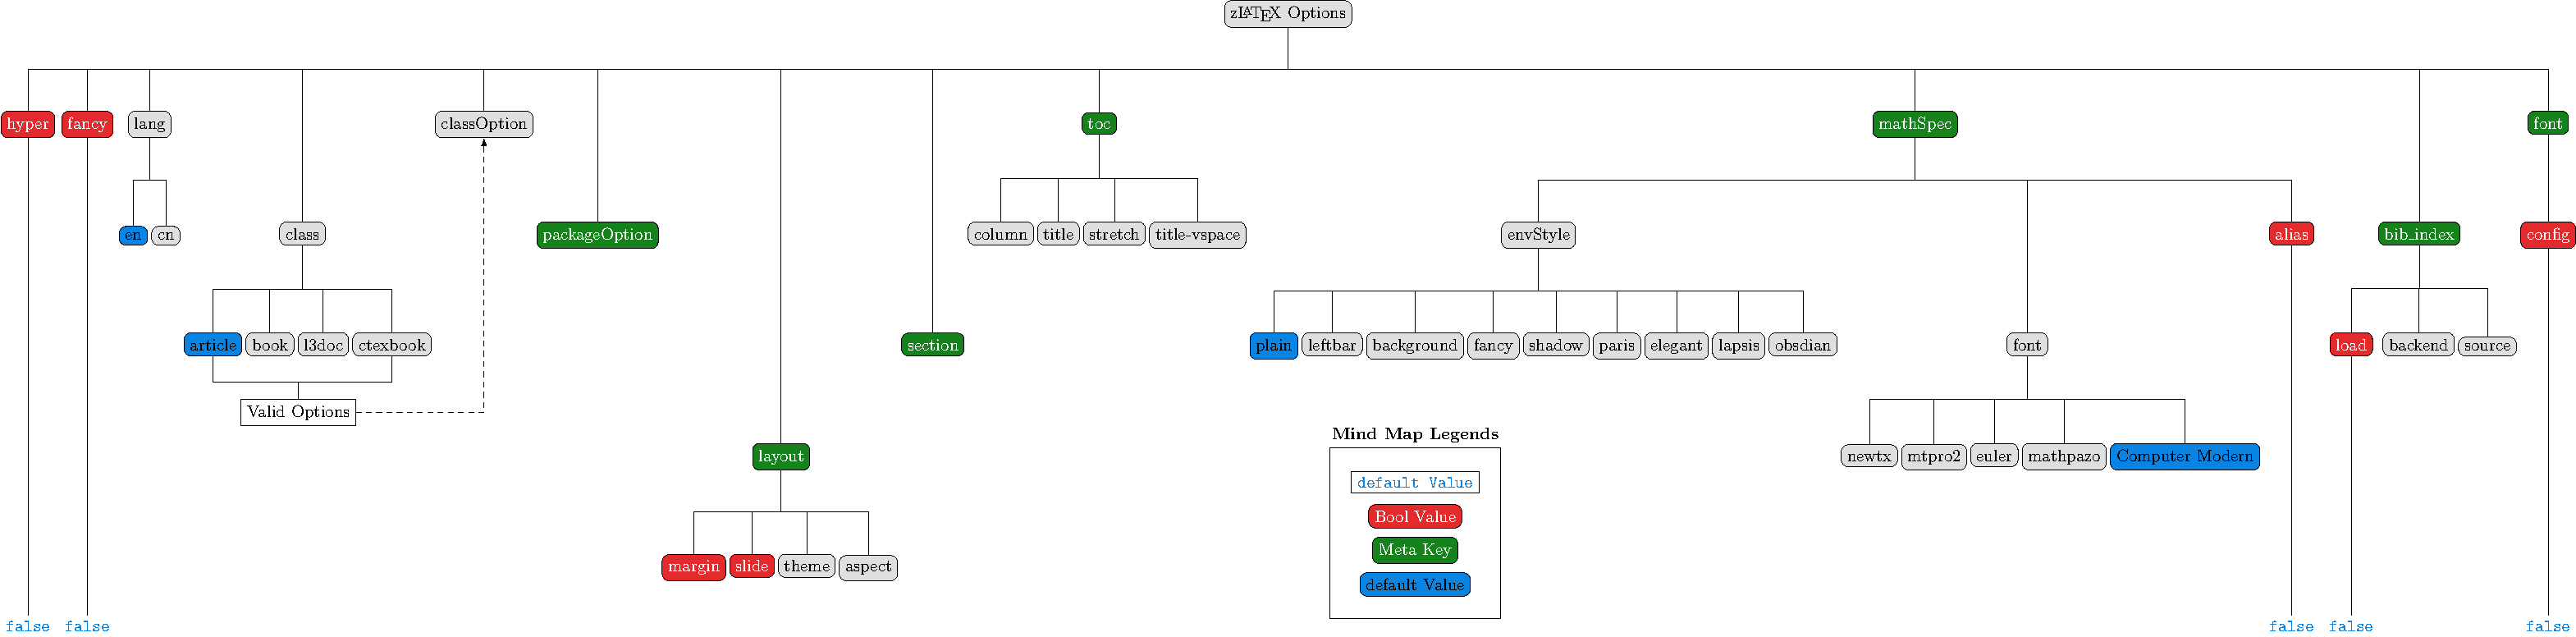
\includegraphics[width=1\linewidth]{zlatex_options.pdf}
  \caption{\zlatex{} 文档类选项示意图}
  \label{fig:zlatex-options}
\end{figure}

总体而言, \zlatex{} 的文档类选项是比较复杂的,对于刚接触本文档类的用户,不必知晓所有的选项配置,因为在默认的
选项配置下, \zlatex{} 已经能够得到一个效果较佳的文档了. 下面我们将详细介绍各个 \meta{key} 的指定方式及其具体含义.

\begin{function}[updated=2024-11-05]{\zlatexloadmodule, \zlatexloadlibrary}
  \begin{syntax}
    \cs{zlatexloadmodule}\marg{module name}
    \cs{zlatexloadlibrary}\marg{library name}
  \end{syntax}
  可以使用这两个命令用于加载 \zlatex 的模块和库,所有的 module 默认全部加载,library 默认全部不加载,
  由用户指定加载. 目前已有的 module 和 library 列表如下:

  \noindent\parbox[t]{.5\linewidth}{
    \noindent \textbf{module 列表:}
    \begin{itemize}
      \item \file{zlatex.module.fontcfg.tex}
      \item \file{zlatex.module.indexref.tex}
      \item \file{zlatex.module.layout.tex}
      \item \file{zlatex.module.pageinfo.tex}
      \item \file{zlatex.module.theme.tex}
      \item \file{zlatex.module.thm.tex}
      \item \file{zlatex.module.titlesec.tex}
      \item \file{zlatex.module.toc.tex}
    \end{itemize}}%
  \parbox[t]{.5\linewidth}{
    \noindent \textbf{library 列表:}
    \begin{itemize}
      \item \file{zlatex.library.fancy.tex}
      \item \file{zlatex.library.mathalias.tex}
      \item \file{zlatex.library.slide.tex}
      \item \file{zlatex.library.theme.tex}
    \end{itemize}}
\end{function}

各个 module 和 library 的加载方式请参见如下示例:
\begin{DocExample}
% \documentclass{zlatex}
\zlatexloadlibrary{/\zarg{fancy}/}
\zlatexloadlibrary{/\zarg{mathalias}/}
\zlatexloadlibrary{/\zarg{slide}/}
\zlatexloadlibrary{/\zarg{theme}/}
\end{DocExample}

你当然可以编写一个你自己的 module, 不妨假设其名称为 \meta{moduleA}; 将此文件命名为 \texttt{zlatex.module.\meta{moduleA}.tex}, 
然后将其放入路径 \meta{z\TeX}\file{/module/} 下,最后使用如下命令加载此 module:
\begin{DocExample}
\zlatexloadmodule{/\meta{moduleA}/}
\end{DocExample}

\begin{function}[rEXP, updated=2024-11-05]{lang}
  \begin{syntax}
    lang=\meta{cn, \zdefault*{en}}
  \end{syntax}
  \zlatex{} 目前仅对中英文做了适配,对于法语仅有部分支持. 根据不同的文档类语言,\zlatex{}会加载不同的和语言相关的
  宏包\index{language packages},不同\meta{lang}设置下, 宏包的加载情况为:
\end{function}
\begin{table}[!htb]
  \begin{tblr}{
    colspec={|X[1, c]|X[1.5, c]|X[1, c]|X[1, c]|X[1, c]|},
    rowspec={|Q[m]|Q[m]|}
  }
  lang=en & \pkg{inputenc}(pdftex) & \pkg{fontenc} & \pkg{babel} & \pkg{microtype} \\
  lang=cn & \pkg{fontspec} & \pkg{ctex} \\
  \end{tblr}
  \caption{\zlatex{} 文档类语言宏包}
  \label{tab:lang-package}
\end{table}

\begin{function}[rEXP, updated=2024-11-05]{hyper}
  \begin{syntax}
    hyper=\meta{true, \zdefault*{false}} 
  \end{syntax}
  是否开启文档内部的超链接以及 PDF 书签,默认为\zlatexVerb{false}. 建议在最后的成稿中启用此选项,在草稿
  阶段置为 \zlatexVerb{false} 可以加快文档的编译速度.
\end{function}

\begin{function}[rEXP, updated=2024-11-05]{fancy}
  \begin{syntax}
    fancy=\meta{true, \zdefault*{false}} 
  \end{syntax}
  此选项用于控制文档的外观,包括章节样式,定理类环境样式,默认为\zlatexVerb{false}. 
\end{function}

\begin{function}[rEXP, updated=2024-11-05]{class}
  \begin{syntax}
    class=\meta{\zdefault*{article}, book, ctexbook} 
  \end{syntax}
  此选项用于指定加载的基文档类,默认为 \cls{article}. 在加载 \cls{ctexbook}文档类后可以使用此文档类
  提供的 \cmd{\ctexset\{\}} 命令进行相关选项的配置. 
\end{function}

\begin{function}[rEXP, updated=2024-11-05]{classOption}
  \begin{syntax}
    classOption=\meta{class options} 
  \end{syntax}
  此选项接受一个键值对, 用于传递基文档类选项,针对默认的 \cls{article} 文档类,此项为\zlatexVerb{oneside, 12pt}. 一个简单的 
  设置样例:
\begin{DocExample}
\documentclass[
  class=article,
  classOption={10pt, leqno, a4paper},
]{zlatex}
\end{DocExample}
\end{function}

\begin{function}[rEXP, updated=2024-11-20]{packageOption}
  \begin{syntax}
    packageOption=\meta{key-value} 
  \end{syntax}
  此选项接受一个键值对, 用于给不同宏包传递选项, 使用样例:
\end{function}
\begin{DocExample}
\documentclass[
  packageOption={
    fontspec=quiet, 
    ctex={scheme=plain, punct=quanjiao},
  },
]{zlatex}
\end{DocExample} 

\begin{function}[updated=2024-12-25]{toc}
  \begin{syntax}
    toc=\meta{key-value}
  \end{syntax}
  此选项用于设置目录的样式,所有可选配置项如下:
\end{function}
\begin{DocExample}
\zlatexSetup{
  toc={
    column=/\meta{int\zdefault{1}}/,
    title=/\meta{tl\zdefault{Contents}}/,
    title-vspace=/\meta{dim\zdefault{-2em}}/,
    stretch=/\meta{float\zdefault{1}}/
  }
}
\end{DocExample}
若上述的 $\meta{column} \ge 2$, 那么 \zlatex{} 会自动加载\pkg{multicol}宏包. 注意: 由于在 \LaTeX{} 中,文档类选项不能含有控制序列,所以如果上述的 \meta{toc} 的某一个子项中含有控制序列,
那么务必通过命令 \cmd{\zlatexSetup} 进行设置, 示例如下:
\begin{DocExample}
\zlatexSetup{
  toc={
      title=\hfill\large\normalfont CONTENTS {\sffamily\small NEW}\hfill
    }
}
\end{DocExample}

\begin{function}[rEXP, updated=2024-12-06]{font}
  \begin{syntax}
    font = \meta{true, \zdefault*{false}}
  \end{syntax}
  此选项目前在实验性阶段,主要用于字体配置, 默认为\zlatexVerb{false}. 在启用此选项后,\zlatex{} 会自动加载
  \pkg{fontspec} 宏包,此时需更换引擎为\hologo{XeLaTeX} 或者 \hologo{LuaLaTeX}.
\end{function}

\begin{function}[rEXP, updated=2024-11-05]{layout}
  \begin{syntax}
    layout=\meta{key-value}
  \end{syntax}
  设置文档布局,所有可选配置项如下:
\end{function}
\begin{DocExample}
\documentclass[
  layout={
    margin=/\meta{bool\zdefault{false}}/,
    slide=/\meta{bool\zdefault{false}}/,
    aspect=/\meta{float|float\zdefault{12:9}}/,
    theme=/\meta{str\zdefault{AnnArborDefault}}/
  },
]{zlatex}
\end{DocExample}
在加载 \file{slide} library 后, 如果设置\meta{slide=true}, 那么此时即可把文档转为 slide 模式。

\begin{function}[updated=2024-12-05]{bib_index}
  \begin{syntax}
    bib_index=\meta{key-value}
  \end{syntax}
  此选项用于控制文档是否生成索引和参考文献,所有可用的选项为:
\begin{DocExample}
\zlatexSetup{
  bib_index={
    load=/\meta{bool\zdefault{false}}/,
    source=/\meta{str\zdefault{ref.bib}}/,
    backend=/\meta{str\zdefault{biber}}/
  }
}
\end{DocExample}
\meta{load} 用于控制是否加载 \pkg{biblatex} 宏包, 默认为 \zlatexVerb{false}; \meta{source} 用于指定参考文献源文件, 默认
文件名为:\file{ref.bib}; \meta{backend} 用于指定参考文献的后端,默认为 {biber}.
\end{function}

\begin{function}[updated=2024-11-05]{mathSpec}
  \begin{syntax}
    mathSpec=\meta{key-value}
  \end{syntax}
  此键用于配置数学排版相关选项. 所有可用的选项为:
\end{function}
\begin{DocExample}
\zlatexSetup{
  mathSpec={
    alias=/\meta{bool\zdefault{false}}/,
    envStyle=/\meta{tl\zdefault{plain}}/,
    font=/\meta{choice\zdefault{ncmrm}}/
  }
}
\end{DocExample}

\meta{alias} 默认为\zlatexVerb{false}, 当置为\zlatexVerb{true} 时,\zlatex{} 会加载\file{mathalias}库, 其中包含一系列
命令的简写声明, 如 \cmd{\ZZ} 代替 \zlatexVerb{\mathbb{Z}}; \meta{envStyle} 用于指定数学环境的样式, 默认为 \zlatexVerb{plain},
为了编译速度考虑,\zlatex{} 在预定了一系列环境的同时,也在 \file{theme} 库中声明了其它样式. 样式列表如下:

\noindent\parbox[t]{.5\linewidth}{
\noindent \textbf{\pkg{thm} module 定义样式}:
\begin{itemize}
  \item plain 
  \item background
  \item leftbar 
  \item fancy 
\end{itemize}}%
\parbox[t]{.5\linewidth}{
\noindent \textbf{\pkg{theme} library 定义样式}:
\begin{itemize}
  \item shadow
  \item paris 
  \item elegant
  \item obsidian
  \item lapsis
\end{itemize}}

\meta{font} 用于指定数学公式字体,预定义的字体有:\zlatexVerb{newtx, euler, mtpro2, mathpazo}. 其中 \zlatexVerb{mtpro2}
为付费字体,需用户手动安装.


\clearpage
\section{杂项}
本小节会列举部分在 \cls{zlatex} 源文件中定义的命令, 这部分命令未迁移到任何的 module 或者是 library 中.

\begin{function}[updated=2024-11-05]{\zlatexVerb}
  \begin{syntax}
    \cs{zlatexVerb}\oarg{format}\marg{item}
  \end{syntax}
  此命令和 \hologo{LaTeX2e} 中的 \cmd{\verb} 类似,用于输出控制序列名称. 和后者类似,此命令也不能作为
  任何控制序列的参数. \meta{format} 用于指定控制序列的打印格式, 默认为 \zlatexVerb{\texttt}. 一个使用
  样例如下:
\end{function}
\begin{DocExample}*
  \zlatexVerb{\alpha + \beta}\par
  \zlatexVerb[\textsf]{\alpha + \beta}
\end{DocExample}

\begin{function}[updated=2024-11-05]{\zlatexCounterWith}
  \begin{syntax}
    \cs{zlatexCounterWith}\marg{child}\marg{parent}
  \end{syntax}
  此命令用于给一个计数器添加一个父计数器, 当 \meta{parent} 计数器增加时,\meta{child} 计数器会自动重置.
  本命令为 \cmd{\@addtoreset} 的封装.
\end{function}

\begin{function}[updated=2024-11-05]{\zlatexFramed}
  \begin{syntax}
    \cs{zlatexFramed}\oarg{color}\marg{name}
  \end{syntax}
  此命令用于创建一个类似 MarkDown 中引用环境, \meta{color} 表示环境 \meta{name} 的默认颜色,在使用环境
  \meta{name} 时可以更改 \meta{color} 这一默认的可选参数. 一个使用样例如下:
\end{function}
\begin{DocExample}*
  \zlatexFramed[red]{ref}
  \begin{ref}This is a simple ref env.\end{ref}
  \begin{ref}[green]This is a simple ref env.\end{ref}
\end{DocExample}


\begin{function}[updated=2024-12-05]{\_zlatex_quad_dim}
  \begin{syntax}
    \cs{_zlatex_quad_dim}
  \end{syntax}
  此命令表示当前文档中一个空格的宽度.
\end{function}


\clearpage
\section{Modules}
本节对应的所有 module 默认自动加载,用户仍可以通过命令 \cmd{\zlatexloadmodule} 调用自己编写的 module.

\subsection{fontcfg}
本模块主要用于配置 \zlatex{} 的字体, 尽管 \pkg{fontspec} 和 \pkg{unicode-math} 已经在很大程度上
简化了字体的配置,但是对于一些用户来说,仍然会感到困扰. 本模块的目的就是为了简化字体的配置,让普通的
\LaTeX{} 用户也能够方便的配置字体, 用上自己喜欢的字体. 

\begin{function}[updated=2024-12-05]{\Cinzel}
  \begin{syntax}
    \cmd{\Cinzel}
  \end{syntax}
  本命令用于临时切换 Cinzel 字体(此时需使用 \hologo{XeLaTeX} 或 \hologo{LuaLaTeX}), 本字体在 \meta{fancy}\zlatexVerb{=true} 时,会自动应用于 chapter 页的字体.
\end{function}

\begin{function}[updated=2024-12-05]{\blacktriangleright}
\begin{syntax}
  \cs{blacktriangleright}
\end{syntax}
本命令(符号)来自 AMSb 字体, \meta{slot}\zlatexVerb{="49}. 主要用于在 \meta{slide}\zlatexVerb{=true} 时对此符号进行 Patch.
\end{function}


\clearpage
\subsection{indexref}
本模块主要用于给文档增加索引,参考文献以及超链接支持, 通过本模块,用户可以方便的添加索引, 参考文献以及超链接.

% \makeatletter
\begin{function}[added=2024-12-05]{\hyper@anchor}
  \begin{syntax}
    \cs{hyper@anchor}\marg{destination name}
  \end{syntax}
  此命令用于创建一个超链接锚点, \meta{destination name} 作为后续超链接命令的跳转目标.
\end{function}


\begin{function}[added=2024-12-05]{\hyper@link}
  \begin{syntax}
    \cmd{\hyper@link}\marg{context}\marg{destination name}\marg{link text}
  \end{syntax}
  此命令用于创建一个超链接, \meta{link text} 本身作为一个超链接对象,点击\meta{link text} 即可跳转到对
  应的 \meta{destination name}. \meta{context} 表示此链接所属的类型, 默认有: \texttt{link, url, cite} 三种类型.
\end{function}

\begin{function}[added=2024-12-05]{\hyper@linkstart}
  \begin{syntax}
    \cmd{\hyper@linkstart}\marg{context}\marg{destination name}
  \end{syntax}
  此命令用于开启一个超链接\textbf{域}, 在此\textbf{域}中可以是任意的文本或其它图片对象. 此命令需结合后续的
  \cmd{\hyper@linkend} 命令使用,此二命令可以和上述的 \cmd{\hyper@link} 命令基本等效.
\end{function}


\begin{function}[added=2024-12-05]{\hyper@linkend}
  \begin{syntax}
    \cmd{\hyper@linkend}
  \end{syntax}
  用于结束由 \cmd{\hyper@linkstart} 开启的\textbf{域}.
\end{function}


\begin{function}[added=2024-12-05]{\MakeLinkTarget,\MakeLinkTarget*}
  \begin{syntax}
  \cs{MakeLinkTarget}\oarg{prefix}\marg{counter}
  \cs{MakeLinkTarget}*\marg{target}
  \end{syntax}
  此二命令用于在用户层面创建超链接跳转目标,其中 \meta{prefix} 和 \meta{counter} 可以作为命令
  \cmd{\hyper@link} 的参数使用. \meta{counter} 可以为 \texttt{chapter, section, subsection} 等.
  针对 \cs{MakeLinkTarget*}, 其中 \meta{target} 可以为任意的 Unicode 文本(但为了兼容性考虑,请尽量使用 ASCII 字符).
\end{function}


\begin{function}[added=2024-12-05]{\LinkTargetOn, \LinkTargetOff}
  \begin{syntax}
    \cs{LinkTargetOn}
    \cs{LinkTargetOff}
  \end{syntax}
  此命令常在一个局部中用于取消由 \cs{MakeLinkTarget} 或 \cs{refstepcounter} 创建的超链接. 在使用 
  \cs{LinkTargetOff} 后,你仍然可以在一个局部里重新启用超链接然后创建对应的 Target, 示例如下:
\end{function}
\begin{DocExample}
\LinkTargetOff  % suppress anchor in internal refstepcounter
...
\refstepcounter{...}
...
{\LinkTargetOn\MakeLinkTarget*{mytarget}} % create manual anchor for future reference
...
\LinkTargetOn
\end{DocExample}


\begin{function}[added=2024-12-05]{\NextLinkTarget}
  \begin{syntax}
    \cs{NextLinkTarget}\marg{target}
  \end{syntax}
  此命令设置下一个由 \cs{MakeLinkTarget} 或 \cs{refstepcounter} 创建的 target. 此命令的作用和 
  \cs{hypersetup} 中的 \cmd{next-anchor} 类似.
\end{function}
% \makeatother


\begin{function}[added=2024-12-05]{\SetLinkTargetFilter}
  \begin{syntax}
    \cs{SetLinkTargetFilter}\marg{filter}
  \end{syntax}
  此命令用于给当前文档中所有的 Link Target 添加一个前缀,此命令在合并多个不同的 PDF 时是十分有用的. 
\end{function}


\clearpage
\subsection{layout}
本模块主要用于设置文章布局,包括纸张大小,页边距等.


\clearpage
\subsection{pageinfo}
本模块主要包含与页面生成以及页面标注相关(页眉页脚)的命令, 如 \cmd{\maketitle},\-\cmd{\zlatexPageMask}; 
通过本模块,用户可以方便的制作自己的独特页面样式以及添加水印.

\begin{function}[updated=2024-11-05]{\orimaketitle}
  \begin{syntax}
    \cs{orimaketitle}
  \end{syntax}
  \cs{maketitle} 的原始形式.
\end{function}

\begin{function}[updated=2024-11-05]{\maketitle}
  \begin{syntax}
    \cs{maketitle}
  \end{syntax}
  \zlatex{} 对原始的 \cs{maketitle} 进行了重定义,以适应不同的文档类和页面布局.
\end{function}

\begin{function}[added=2024-12-05]{\Maketitle}
  \begin{syntax}
    \cs{Maketitle}\oarg{margin\zdefault{1in}}
  \end{syntax}
  此命令会忽略所有的文档类选项或者是页面布局,在新的页面布局中插入 \cmd{\maketitle} 的原始定义, \meta{margin} 
  表示新的页面布局的 margin, 默认为 \texttt{1in}. 此命令的实现为:
\end{function}
\begin{DocExample}
\newcommand\Maketitle[1][1in]{
  \newgeometry{margin=#1}
  \orimaketitle
  \restoregeometry
}
\end{DocExample}


\begin{function}[updated=2024-11-05]{\frontmatter, \mainmatter}
  \begin{syntax}
    \cs{frontmatter}
    \cs{mainmatter}
  \end{syntax}
  此二命令用于设置文档的前言和正文部分,在 \zlatex{} 中这两个命令已经被重定义,当加载的 \meta{class} 为 \cls{book} 或 \cls{ctexbook} 时,
  这两个命令会自动处理页眉页脚相关设置.
\end{function}

\begin{function}[updated=2024-12-05]{\__zlatex_page_annotate:nnnnn}
  \begin{syntax}
    \cmd{\__zlatex_page_annotate:nnnnn} \marg{fore/background}
      \marg{position}\marg{anchor}
      \marg{object}\marg{hook range}
  \end{syntax}
  此命令为 \cmd{\zlatexPageMask} 的底层命令, 用户可以依据此命令创建更加具有针对性的水印命令.
\end{function}

\begin{function}[updated=2024-12-05]{\zlatexPageMask, \zlatexPageMask*}
  \begin{syntax}
    \cs{zlatexPageMask}\oarg{key-value}\marg{item}
  \end{syntax}
  命令 \cmd{\zlatexPageMask} 用于给当前页面添加水印,\cmd{\zlatexPageMask*} 用于给当前页面及其之后的所有
  页面添加水印. \meta{item} 可以为一段文字,也可以为一系列的图片(需要使用\cmd\includegraphics 进行导入). 
  \meta{key-value} 所有可用的选项为:
\end{function}
\begin{DocExample}
  \zlatexPageMask[
    layer=/\meta{tl:\zdefault*{background}, foreground}/, 
    position=/\meta{tl:(dim1, dim2)}/,
    label=/\meta{tl:\zdefault*{DEFAULT}}/, 
    anchor=/\meta{tl:\zdefault*{c}, tl, tc, tr, bl, bc, br}/
  ]{/\meta{item}/}
\end{DocExample}
其中\meta{position}以页面的左下角为原点,向上向右为正方向. 注意: \pkg{transparent}宏包仅可以在 \hologo{pdfLaTeX} 和 
\hologo{LuaLaTeX} 下正常工作. 一个简单的示例, 给当前页面添加一个水印:
\begin{DocExample}*
  % \usepackage{tikzlings}
  \zlatexPageMask{
    \transparent{.5}
\includegraphics{latex-logo.pdf};
  }
  \zlatexPageMask[anchor=tr, position={(\zpw, \zph)}]{
    \begin{tikzpicture}[scale=2]
      \marmot
    \end{tikzpicture}
  }
\end{DocExample}
上述的 \cmd{\zpw}, \cmd{\zph} 分别表示当前纸张的宽和高.


\begin{function}[added=2024-12-05]{\zlatexPageMaskRemove}
  \begin{syntax}
    \cs{zlatexPageMaskRemove}\marg{foreground/backgroud}\marg{label}
  \end{syntax}
  此命令用于移除由 \cmd{\zlatexPageMask} 命令添加的页面水印, \meta{label} 即为 \cmd{\zlatexPageMask} 可选
  参数 \meta{key-value} 中 \meta{label} 对应的 value. 如果 \meta{label} 对应的水印并不存在, \zlatex{} 会抛出警告.
\end{function}


\clearpage
\subsection{theme}
本模块主要用于文档装饰,在本模块中定义了一系列的颜色主题,这系列主题可以应用于文章中的各个元素,包括但不限于
章节标题, 定理环境, 超链接跳转,(子)目录样式.

\begin{function}[updated=2024-11-05]{\zlatexColorSetup}
  \begin{syntax}
    \cs{zlatexColorSetup}\marg{key-value}
  \end{syntax}
  当 \meta{hype}\zlatexVerb{=true} 时, 此命令可以用于设置文档中各种元素的色彩, 但仅可在导言区使用. \zlatex{} 把文档
  中的元素分为如下的 3 类:
  \begin{itemize}
    \item 章节标题类: \zlatexVerb{chapter, chapter-rule}
    \item 超链接类: \zlatexVerb{link, cite, url}
    \item 定理环境类: \env{axiom, definition, theorem, proposition, lemma, corollary, proof, example, solution}
  \end{itemize}
  在颜色指定上,\zlatex{} 实现了一套自己的颜色指定方式, 在指定色彩时可以不必要提前定义. 参见如下使用案例:
  \begin{DocExample}
    \zlatexColorSetup{
      chapter = red,
      link = {HTML}{d9d9d9},
      theorem = {RGB}{136, 63, 214}
    }
  \end{DocExample}
\end{function}

\zlatex{} 的默认配色\Footnote{zchapColor 还未整理, 目前只能单独重定义}如下:
\begin{table}[H]
  \begin{tblr}{
    colspec={|X[1.25, c]|X[1, c]|X[1.5, c]|X[1.1, c]|X[1, c]|X[1.1, c]|X[1.65, c]|X[1.65, c]|},
    rowspec={|Q[m]|Q[m]|Q[m]|Q[m]|},
    cells={cmd=\small\env}
  }
    Struct & chapter & chap-rule & link & url & cite  & chap-theme  & slide-theme\\ 
    Color & \block{RoyalRed} & \block{black} & \block{purple}& \block{RoyalRed} & \block{blue} & \block{zchapColor} & \block{Ann-default-I}\\
    MathEnv & axiom & definition & theorem & lemma & corollary & proposition & remark \\  
    Color & \block{zlatex@color@axiom} & \block{zlatex@color@definition} & \block{zlatex@color@theorem} & 
    \block{zlatex@color@lemma}& \block{zlatex@color@corollary}& \block{zlatex@color@proposition}& \block{zlatex@color@remark}\\
  \end{tblr}
  \caption{z\LaTeX{}文档类默认配色}
  \label{tab:zlatex-default-color}
\end{table}

定理类环境的色彩保存于变量 \cmd{zlatex@color@\meta{name}} 中, 其中 \meta{name} 为对应环境的名称. 不推荐用户 使用命令 \cmd{\definecolor}, \cmd{\colorlet} 
直接对这类色彩变量进行重定义, \zlatex{} 鼓励用户通过 \cmd{\zlatexColorSetup} 命令进行色彩的重定义.

\begin{function}[updated=2024-12-05]{\__zlatex_color_set:n}
  \begin{syntax}
    \cmd{\__zlatex_color_set:n} \marg{color spec}
  \end{syntax}
  此命令可以自动解析 \meta{color spec}, 并以此创建或定义对应的色彩. \meta{color spec} 可以为普通的
  预定义色彩名,如 \texttt{red, orange} 等. 亦或者是 \texttt{HTML, RGB, CMYK} 等色彩模型,但此时的格式略有
  不同。此命令仅能在 \cmd{\keys_define:nn} 中使用,新定义的色彩名为 \zlatexVerb{zlatex@color@\l_keys_key_str}. 
  关于参数 \meta{color spec} 的使用,可以参见如下示例:
\end{function}
\begin{DocExample}
\__zlatex_color_set:n {red}
\__zlatex_color_set:n {{HTML}{393D44}}
\end{DocExample}


\clearpage
\subsection{thm}
本模块主要用于定理类以及证明类数学环境定制. 本模块提供了丰富的接口以及选项,与此同时本模块提供了丰富的
Hook, 方便用户直接对环境进行操作.


\begin{function}[updated=2024-11-05]{\zlatexThmLang}
  \begin{syntax}
    \cs{zlatexThmLang}\marg{lang}
  \end{syntax}
  此命令用于设置定理类环境的名称, 目前支持 \zlatexVerb{cn, en, fr} 三种语言. 此命令仅能在文档的导言区使用, 但为了说明此命
  令的使用方法,在本手册中,此命令的定义被临时改变了. 一个使用样例如下:
\end{function}
\begingroup
\begin{DocExample}*
  \begin{theorem}[AAA-1]
    This is a theorem AAA-1.
  \end{theorem}
  \zlatexThmLang{fr}
  \begin{theorem}[BBB-1]
    This is a france theorem BBB-1.
  \end{theorem}
  \zlatexThmLang{en}
  \begin{theorem}[CCC-1]
    This is a english theorem CCC-1.
  \end{theorem}
\end{DocExample}
\endgroup


\zlatexThmStyle{background}
\begin{function}[updated=2024-12-25]{\zlatexThmCreate}
  \begin{syntax}
    \cs{zlatexThmCreate}\marg{type}\marg{spec}
  \end{syntax}
  根据 \meta{spec} 创建一系列类型为 \meta{type} 的定理环境, 如果对应的环境已存在,则覆盖其原有的定义. 
  \meta{type} 可选\zlatexVerb{theorem, proof}两种类型, 针对 \meta{spec}, 请参见下面的使用样例:
\end{function}
\begin{DocExample}*
  \zlatexThmCreate{theorem}{Zaxiom, Ztheorem=Thm|{HTML}{a0d911}, Zproposition=Prop|blue}
  \zlatexThmCreate{proof}{Zproof, Zexample=EXAMPLE|red, Zsolution=Solution|}
  \begin{Zproof}[AAA-2]
    This is an proof AAA-2.
  \end{Zproof}
  \begin{Zexample}[BBB-2]
    This is an example.
  \end{Zexample}
  \begin{Ztheorem}[CCC-2]
    This is a theorem
  \end{Ztheorem}
\end{DocExample} 
\cmd{\zlatexThmCreate} 仅可在导言区使用. 但为了说明此命令的使用方法,在本手册中,此命令的定义被临时改变了.
和前面的 \cmd{\zlatexColorSetup} 类似, 在指定色彩时可以不必要提前定义.
% 注意: \meta{spec} 中类似 \cmd{Zsolution=Solution|} 这样的定义是不合法的, 此定义最后的 \cmd{|} 应被移除.
\zlatexThmStyle{plain}

\begin{function}[EXP, updated=2024-11-05]{\zlatexThmNumber}
  \begin{syntax}
    \cs{zlatexThmNumber}
  \end{syntax}
  此命令表示对应环境的编号, 类似于 \pkg{amsthm} 中的 \cmd{\thmnumber}. 用户不应在除 \cmd{\zlatexThmTitleFormat} 外的
  任何地方使用, 在此命令之外, 此命令输出的内容无任何实际意义.
\end{function}

\begin{function}[EXP, updated=2024-11-05]{\zlatexThmName}
  \begin{syntax}
    \cs{zlatexThmName}
  \end{syntax}
  此命令表示对应环境的名称, 类似于 \pkg{amsthm} 中的 \cmd{\thmname}. 用户不应在除 \cmd{\zlatexThmTitleFormat} 外的
  任何地方使用, 在此命令之外, 此命令输出的内容无任何实际意义.
\end{function}

\begin{function}[EXP, updated=2024-12-05]{\zlatexThmNote}
  \begin{syntax}
    \cs{zlatexThmNote}\marg{prefix}\marg{suffix}
  \end{syntax}
  此命令表示对应环境的注释, 类似于 \pkg{amsthm} 中的 \cmd{\thmnote}. 用户不应在除 \cmd{\zlatexThmTitleFormat} 外的
  任何地方使用, 在此命令之外, 此命令输出的内容无任何实际意义.
\end{function}

\begin{function}[EXP, updated=2024-11-05]{\zlatexThmTitle}
  \begin{syntax}
    \cs{zlatexThmTitle}
  \end{syntax}
  此命令表示对应环境的标题, 包含 \cmd{\zlatexThmNumber}, \cmd{\zlatexThmName}, \cmd{\zlatexThmNote} 三
  部分. 具体的格式可以使用 \cmd{\zlatexThmTitleFormat} 进行指定.
\end{function}
% \clearpage


\begin{function}[updated=2024-11-05]{\zlatexThmTitleSwitch}
  \begin{syntax}
    \cs{zlatexThmTitleSwitch}
  \end{syntax}
  此命令用于切换 \cmd{\zlatexThmTitle} 是否显示, 在自定义环境样式时比较有用. 用户不应该对此命令
  进行直接的调用.
\end{function}
\begin{DocExample}*
  \begin{theorem}[AAA-3]
    This is a theorem AAA-3.
  \end{theorem}
  \zlatexThmStyleNew{
    ZZZ={begin=, end=, option=\zlatexThmTitleSwitch},
  }
  \zlatexThmStyle{ZZZ}
  \begin{theorem}[BBB-3]
    This is a theorem BBB-3.
  \end{theorem}
\end{DocExample}
关于命令 \cmd{\zlatexThmStyle} 的使用可以参见下面的说明.

\begin{function}[updated=2024-11-05]{\zlatexThmTitleFormat, \zlatexThmTitleFormat*}
  \begin{syntax}
    \cs{zlatexThmTitleFormat}\marg{format}
  \end{syntax}
  此命令用于指定 \cmd{\zlatexThmTitle} 的格式, 默认格式为:
  \begin{DocExample}
    \zlatexThmName\ \zlatexThmNumber\ \zlatexThmNote{(}{)}
  \end{DocExample}
\end{function}


\begin{function}[updated=2024-12-05]{\zlatexThmNoteEmptyTF}
  \begin{syntax}
    \cs{zlatexThmNoteEmptyTF}\marg{true code}\marg{false code}
  \end{syntax}
  此命令用于判断 \cmd{\zlatexThmNote} 是否为空, 如果为空则执行 \meta{true code}, 否则执行 \meta{false code}.
  这个命令在自定义 \cmd{\zlatexThmTitle} 时很有用. 一个使用样例(\zlatex{} 内置的 \zlatexVerb{obsidian} 定理样式对应的 format):
\end{function}
\begin{DocExample}
\zlatexThmTitleFormat*{\bfseries
  \zlatexThmName\ \zlatexThmNumber
  \zlatexThmNoteEmptyTF{}{\\}
  \zlatexThmNote{}{}
}
\end{DocExample}


\begin{function}[updated=2024-12-05]{\zlatexThmBefore}
  \begin{syntax}
    \cs{zlatexThmBefore}\marg{code\zdefault{\cs{par}}}
  \end{syntax}
  此命令用于把 \meta{code} 置于每个环境(命令 \cmd{\__zlatex_thm_warp_start:nnnn})之前, 默认为 \cs{par}.
  用户可以把 \meta{code} 置为空或者是 \cs{noindent} 以取消段落缩进.
\end{function}

\begin{function}[updated=2024-11-05]{\qedsymbol}
  \begin{syntax}
    \cs{qedsymbol}
  \end{syntax}
  此命令用于输出证明环境的结束符号, 默认为 $\square$.
\end{function}


\begin{function}[updated=2024-11-05]{\zlatexThmCnt}
  \begin{syntax}
    \cs{zlatexThmCnt}\marg{key-value}
  \end{syntax}
  此命令用于定义数学类环境的计数器, 仅能在导言区使用, 但为了说明此命令的使用方法,
  在本手册中,此命令的定义被临时改变了. 所有可用的选项为:
\end{function}
\begin{DocExample}
  \zlatexThmCnt{
    parent=/\meta{counter\zdefault{section}}/,
    share=/\meta{bool\zdefault{false}}/
  }
\end{DocExample}
\meta{parent} 用于指定计数器的父计数器, 默认父计数器为 \zlatexVerb{section}; 当父计数器更新时,此环境的计数器便会重置; \meta{share}
用于控制所有的定理类环境是否共用一个计数器,默认不共用.


\begin{function}[updated=2024-11-05]{\zlatexThmColorSetup}
  \begin{syntax}
    \cs{zlatexThmColorSetup}\marg{key-value}
  \end{syntax}
  此命令和 \cmd{\zlatexColorSetup} 类似,但其仅用于对数学环境的色彩设置,且仅能在导言区使用. 
  所有合法的 \meta{key} 选项请参见 \zlatex{} 文档类选项 \cmd{mathSpec} 中的数学环境.
\end{function}

\begin{function}[updated=2024-11-05]{\zlatexThmStyle}
  \begin{syntax}
    \cs{zlatexThmStyle}\marg{style}
  \end{syntax}
  此命令用于设置定理类环境的样式, 仅能在导言区使用. 可用的 \meta{style} 请参见 \meta{mathSpec} 的说明.
  一个基本的使用样例:
\end{function}
\begin{DocExample}*
  \begin{theorem}[AAA-4]
    This is a theorem AAA-4.
  \end{theorem}
  \zlatexThmStyle{fancy}
  \begin{theorem}[BBB-4]
    This is a fancy theorem BBB-4.
  \end{theorem}
\end{DocExample}
\zlatexThmStyle{plain}

\begin{function}[updated=2024-12-05]{\zlatexThmStyleNew}
  \begin{syntax}
    \cs{zlatexThmStyleNew}\marg{key-value}
  \end{syntax}
  此命令用于定义新的定理类环境的样式, 仅能在导言区使用. 调用格式为:
\end{function}
\begin{DocExample}
  \zlatexThmStyleNew{
    /\meta{style A}/={
      begin=/\meta{begin code 1}/, 
      end=/\meta{end code 1}/, 
      option=/\meta{option 1}/,
      preamble=/\meta{preamble code 1}/
    },
    /\meta{style B}/={
      begin=/\meta{begin code 2}/, 
      end=/\meta{end code 2}/, 
      option=/\meta{option 2}/,
      preamble=/\meta{preamble code 2}/
    },
    ...
  }
\end{DocExample}
在声明对应的 \meta{style} 后,使用命令 \cmd{\zlatexThmStyle}\marg{style} 进行切换.


\begin{function}[updated=2024-11-05]{\zlatexThmHook, \zlatexThmHook*}
  \begin{syntax}
    \cs{zlatexThmHook}\marg{key-value}
    \cs{zlatexThmHook*}\marg{key-value}
  \end{syntax}
  此命令用于给已有的定理类环境 Hook 中添加代码, 已有的 Hook: \zkey{zlatex/thm/before, zlatex/thm/begin,
  zlatex/thm/end, zlatex/thm/after}. \cs{zlatexThmHook} 只应用于下一个环境, \cs{zlatexThmHook*} 会应用于接下来的
  所有环境. 各个 Hook 的位置分布如下:
\end{function}
\begin{DocExample}[@@]
(zlatex/thm/before) --> (warper begin) 
  --> (thm-title)   --> (zlatex/thm/begin) 
  --> (thm-content) --> (zlatex/thm/end) --> 
(warper end) --> (zlatex/thm/after)
\end{DocExample}

这两个命令不支持手动设置\meta{label}, 针对于 \cmd{\zlatexThmHook*}, \zlatex{} 会自动设置 \meta{label}, 其格式
为 \cmd{thm-hook.\meta{Hook Index}}. 针对 \meta{key}, 所有合法的选项为:\zkey{before, begin, end, after}, 
一个使用样例如下:
\begin{DocExample}*
\begin{theorem}[AAA-5]
  This is a theorem AAA-5.
\end{theorem}
\zlatexThmHook{before=ZZa\ , begin=ZZb\ ,}
\begin{theorem}[BBB-5]
  This is a theorem BBB-5.
\end{theorem}
\end{DocExample}

\begin{function}[updated=2024-12-05]{\zlatexThmToc}
  \begin{syntax}
    \cs{zlatexThmToc}\oarg{stretch}
  \end{syntax}
  此命令用于打印定理类环境的目录, \meta{stretch} 为任意非负的浮点数, 用于指定定理目录的 stretch 值. 使用样例如下:
\end{function}
\begin{DocExample}*
\zlatexThmToc[1.25]
\begin{proposition}[AAA-6]proposition AAA-6\end{proposition}
\begin{lemma}[BBB-6]lemma BBB-6\end{lemma}
\begin{corollary}[CCC-3]corollary CCC-3\end{corollary}
\end{DocExample}

\begin{function}[updated=2024-12-05]{\zlatexThmTocAdd}
  \begin{syntax}
    \cs{zlatexThmTocAdd}\oarg{key-value}\marg{counter}
  \end{syntax}
  此命令用于向定理类环境目录中添加条目, \meta{counter} 为计数器名, 可以为 \zlatexVerb{section}, 
  \zlatexVerb{subsection} 等. \meta{key-value} 为可选参数, 用于指定所添加的条目的其它信息. 一个使用样例如下:
\end{function}
\begin{DocExample}
\zlatexThmTocAdd[name=SEC-NAME]{section}
\end{DocExample}


\begin{function}[updated=2024-12-05]{\zlatexThmTocLevel}
  \begin{syntax}
    \cs{zlatexThmTocLevel}\marg{depth}
  \end{syntax}
  此命令用于设置定理类环境目录的最大深度, 仅能在导言区使用, 但为了说明此命令的使用方法, 本手册中此命令
  的定义被临时改变了. \meta{depth} 为一个 $\ge 1$ 的整数.
\end{function}

\begin{function}[updated=2024-12-05]{\zlatexThmTocPrefix}
  \begin{syntax}
    \cs{zlatexThmTocPrefix}\marg{prefix}
  \end{syntax}
  此命令用于所有定理类环境目录中所有条目的共同前缀, 默认为空. 
\end{function}

\begin{function}[updated=2024-12-05]{\zlatexThmTocSymbol}
  \begin{syntax}
    \cs{zlatexThmTocSymbol}\marg{key-value}
  \end{syntax}
  此命令用于分别设置所有定理类环境名在目录中的前缀, 仅能在导言区使用, 但为了说明此命令的使用方法, 本手册中此命令
  的定义被临时改变了. 所有可用的选项为:
\end{function}
\begin{DocExample}
\zlatexThmTocSymbol{
  /\meta{axiom\zdefault{ \textbf{A}\; }}/,
  /\meta{definition\zdefault{ \textbf{D}\; }}/,
  /\meta{theorem\zdefault{ \textbf{T}\; }}/,
  /\meta{lemma\zdefault{ \textbf{L}\; }}/,
  /\meta{corollary\zdefault{ \textbf{C}\; }}/,
  /\meta{proposition\zdefault{ \textbf{P}\; }}/,
  /\meta{remark\zdefault{ \textbf{R}\; }}/,
}
\end{DocExample}


\begin{function}[updated=2024-12-05]{\zlatexThmTocSymbolClear}
  \begin{syntax}
    \cs{zlatexThmTocSymbolClear}
  \end{syntax}
  此命令用于清除所有由命令 \cmd{\zlatexThmTocSymbol} 指定的定理类环境名在目录中的前缀, 自然不包括
  由 \cmd{\zlatexThmTocPrefix} 指定的前缀.
\end{function}


\clearpage
% \newpage
\subsection{titlesec}
本模块的用于定义章节标题样式, 目的是实现 \pkg{titlesec} 和 \pkg{titletoc} 中的所有功能,
使其能作为上述两宏包的一个可选替代. 后续可能会与 \pkg{toc} module 合并.



\clearpage
\subsection{toc}
本模块主要用于自定义目录格式, 目前基于 \pkg{titletoc}, 后续可能会与 \pkg{titlesec} module 合并.

\begin{function}[updated=2024-11-05]{\zlatexPartialToc}
  \begin{syntax}
    \cs{zlatexPartialToc}\oarg{depth\zdefault{2}}
  \end{syntax}
  此命令用于输出每一个章节对应的子目录, 此命令目前基于 \pkg{titletoc} 宏包. \meta{depth} 用于指定子目录最大深度,
  默认为 2.
\end{function}

\begin{function}[updated=2024-11-05]{\zlatexStopPartialToc}
  \begin{syntax}
    \cs{zlatexStopPartialToc}\marg{\zdefault*{chapters},section}\marg{counter}
  \end{syntax}
  此命令用于结束子目录的搜集,一般情况下,用户不应该使用此命令.
\end{function}


\clearpage
\section{Libraries}
本节主要介绍 \zlatex{} 中提供的各类 library,这些 library 用于优化用户 \LaTeX{} 的文档书写和阅读体验。
部分 library 是对 \zlatex{} 中原始功能的增强,但与此同时,文档的编译速度势必会稍微减慢,所以请酌情加载这部分
library. 

所有的 library 均不默认加载,用户需要使用 \cmd{\zlatexloadlibrary}\texttt{\marg{library name}} 手动加载, 
详细的 \meta{library name} 请参见命令 \cmd{\zlatexloadlibrary} 的说明. 

\subsection{fancy}
此 library 用于章节的格式化以及部分的,目前仅对 \cmd{\chapter} 进行了重定义. 如果此时 \meta{fancy}\texttt{=true},
那么在加载此 library 的同时,\zlatex{} 会同时加载 \pkg{tcolorbox}, \pkg{tikz} 以及 \pkg{tikz} 的 \pkg{calc} 库.

\begin{function}[updated=2024-11-05]{\numSuffix}
  \begin{syntax}
    \cs{numSuffix}\marg{number}
  \end{syntax}
  此命令用于数字的格式化, 其中 \meta{number} 为一个任意的整数, 一个使用样例如下:
\end{function}
\begin{DocExample}*
  \numSuffix{1}, \numSuffix{2}, \numSuffix{25}
\end{DocExample}


\clearpage
\subsection{mathalias}
本模块主要为一系列命令的别名定义, 后文称此为 alias, 用于简化用户在数学环境中的命令输入. 此 libray 建立了以下几个
方面的 alias:
\begin{itemize}
  \item 数学字体命令
  \item 各类箭头
  \item 各类数学算符
  \item 其余常见符号
  \item 自动括号命令(试验阶段)
\end{itemize}

对于自动括号命令,目前还很不成熟,如果不清楚对应的命令原理请勿使用。正对此特性,推荐用于使用 \pkg{pyhsics 2} 
宏包.

\begin{function}[updated=2024-12-05]{\F, \R, \K, \C, \B, \S, \FF}
  \begin{syntax}
    \cs{F}\marg{math char}
    \cs{R}\marg{math char}
    \cs{K}\marg{math char}
    \cs{C}\marg{math char}
    \cs{B}\marg{math char}
    \cs{S}\marg{math char}
    \cs{FF}\marg{math char}
  \end{syntax}
  以上各命令的原始定义: \cmd{\F} 为 \cmd{\boldsymbol}, \cmd{\R} 为 \cmd{\mathrm}, 
  \cmd{\K} 为 \cmd{\mathfrak}, \cmd{\C} 为 \cmd{\mathcal}, \cmd{\B} 为 \cmd{\mathbb},
  \cmd{\S} 为 \cmd{\mathscr}, \cs{FF} 为 \cmd{\mathbf}. 使用示例如下:
\end{function}
\begin{DocExample}*
Normal Version: $\mathbf{A} + \mathrm{A} + \mathfrak{a} + \mathcal{A} + \mathbb{A} + \mathscr{A} + \mathbf{A}$ \\
Alias Version: $\F{A} + \R{A} + \K{a} + \C{A} + \B{A} + \S{A} + \FF{A}$
\end{DocExample}

\begin{function}[updated=2024-12-05]{\ma, \mma}
  \begin{syntax}
    \cs{ma}
    \cs{mma}
  \end{syntax}
  以上各命令的原始定义: \cmd{\ma} 为 \cs{mapsto}, \cmd{\mma} 为 \cs{longmapsto}. 使用示例如下:
\end{function}
\begin{DocExample}*
Normal Version: $a\mapsto b, a\longmapsto b$ \\
Alias Version: $a\ma b, a\mma b$
\end{DocExample}

\begin{function}[updated=2024-12-05]{\la, \La, \nla, \Nla, \lla, \Lla}
  \begin{syntax}
    \cs{la}
    \cs{La}
    \cs{nla}
    \cs{Nla}
    \cs{lla}
    \cs{Lla}
  \end{syntax}
  以上各命令的原始定义: \cmd{\la} 为 \cs{leftarrow}, \cmd{\La} 为 \cs{Leftarrow}, 
  \cmd{\nla} 为 \cs{nleftarrow}, \cmd{\Nla} 为 \cs{nLeftarrow}, \cmd{\lla} 为 \cs{longleftarrow},
  \cmd{\Lla} 为 \cs{Longleftarrow}. 使用示例如下:
\end{function}
\begin{DocExample}*
Normal Version: $a\leftarrow b, a\Leftarrow b, a\nleftarrow b, a\nLeftarrow b, a\longleftarrow b, a\Longleftarrow b$ \\
Alias Version: $a\la b, a\La b, a\nla b, a\Nla b, a\lla b, a\Lla b$.
\end{DocExample}

\begin{function}[updated=2024-12-05]{\ra, \Ra, \nra, \Nra, \rra, \Rra}
  \begin{syntax}
    \cs{ra}
    \cs{Ra}
    \cs{nra}
    \cs{Nra}
    \cs{rra}
    \cs{Rra}
  \end{syntax}
  以上各命令的原始定义: \cmd{\ra} 为 \cs{rightarrow}, \cmd{\Ra} 为 \cs{Rightarrow}, 
  \cmd{\nra} 为 \cs{nrightarrow}, \cmd{\Nra} 为 \cs{nRightarrow}, \cmd{\rra} 为 \cs{longrightarrow},
  \cmd{\Rra} 为 \cs{Longrightarrow}. 使用示例如下:
\end{function}
\begin{DocExample}*
Normal Version: $a\rightarrow b, a\Rightarrow b, a\nrightarrow b, a\nRightarrow b, a\longrightarrow b, a\Longrightarrow b$ \\
Alias Version: $a\ra b, a\Ra b, a\nra b, a\Nra b, a\rra b, a\Rra b$.
\end{DocExample}

\begin{function}[updated=2024-12-05]{\da, \Da, \nda, \Nda, \dda, \Dda}
  \begin{syntax}
    \cs{da}
    \cs{Da}
    \cs{nda}
    \cs{Nda}
    \cs{dda}
    \cs{Dda}
  \end{syntax}
  以上各命令的原始定义: \cmd{\da} 为 \cs{leftrightarrow}, \cmd{\Da} 为 \cs{Leftrightarrow}, 
  \cmd{\nda} 为 \cs{nleftrightarrow}, \cmd{\Nda} 为 \cs{nLeftrightarrow}, \cmd{\dda} 为 \cs{longleftrightarrow},
  \cmd{\Dda} 为 \cs{Longleftrightarrow}. 使用示例如下:
\end{function}
\begin{DocExample}*
Normal Version: $a\leftrightarrow b, a\Leftrightarrow b, a\nleftrightarrow b, a\nLeftrightarrow b, a\longleftrightarrow b, a\Longleftrightarrow b$ \\
Alias Version: $a\da b, a\Da b, a\nda b, a\Nda b, a\dda b, a\Dda b$.
\end{DocExample}


\begin{function}[updated=2024-12-05]{\xla, \xla*, \Xla, \Xla*, \xxla, \xxla*, \xra, \xra*, \Xra, \Xra*, \xxra, \xxra*, \hla, \hla*, \hra, \hra*}
  \begin{syntax}
    \cs{xla}\oarg{above}\parg{below}
    \cs{xla*}\oarg{above}\parg{below}
    \cs{Xla}\oarg{above}\parg{below}
    \cs{Xla*}\oarg{above}\parg{below}
    \cs{xxla}\oarg{above}\parg{below}
    \cs{xxla*}\oarg{above}\parg{below}
    \cs{xra}\oarg{above}\parg{below}
    \cs{xra*}\oarg{above}\parg{below}
    \cs{Xra}\oarg{above}\parg{below}
    \cs{Xra*}\oarg{above}\parg{below}
    \cs{xxra}\oarg{above}\parg{below}
    \cs{xxra*}\oarg{above}\parg{below}
    \cs{hla}\oarg{above}\parg{below}
    \cs{hla*}\oarg{above}\parg{below}
    \cs{hra}\oarg{above}\parg{below}
    \cs{hra*}\oarg{above}\parg{below}    
  \end{syntax}
  以上所有带有 \texttt{*} 命令中的 \meta{above} 参数均会被放入 \cmd{\text} 命令中, 以上命令的原始定义: \cmd{\xla} 为 \cs{xleftarrow}, 
  \cmd{\Xla} 为 \cs{xLeftarrow}, \cmd{\xxla} 为 \cs{xLongleftarrow}, \cmd{\xra} 为 \cs{xrightarrow}, \cmd{\Xra} 为 \cs{xRightarrow},
  \cmd{\xxra} 为 \cs{xLongrightarrow}, \cmd{\hla} 为 \cs{xhookleftarrow}, \cmd{\hra} 为 \cs{xhookrightarrow}. 
  使用示例如下:
\end{function}
\begin{DocExample}*
Normal Version: $\xleftarrow[b]{a} + \xLeftarrow[b]{a} + \xLongleftarrow[b]{a} + \xrightarrow[b]{a} + \xRightarrow[b]{a} + \xLongrightarrow[b]{a} + \xhookleftarrow[b]{a} + \xhookrightarrow[b]{a}$ \\ 
Alias Version: $\xla[a](b) + \Xla[a](b) + \xxla[a](b) + \xra[a](b) + \Xra[a](b) + \xxra[a](b) + \hla[a](b) + \hra[a](b)$ \\
Alias Text Version: $\xla*[a](b) + \Xla*[a](b) + \xxla*[a](b) + \xra*[a](b) + \Xra*[a](b) + \xxra*[a](b) + \hla*[a](b) + \hra*[a](b)$
\end{DocExample}

\begin{function}[updated=2024-12-05]{\A, \E}
  \begin{syntax}
    \cs{A}
    \cs{E}
  \end{syntax}
  以上两个命令分别表示任意和存在符号, 一个使用样例如下:
\end{function}
\begin{DocExample}*
Normal Version: $\forall \varepsilon>0, \exists \delta$ \\
Alias Version: $\A \varepsilon>0, \E \delta$
\end{DocExample}

\begin{function}[updated=2024-12-05]{\ns, \se, \sse}
  \begin{syntax}
    \cs{ns}
    \cs{se}
    \cs{sse}
  \end{syntax}
  以上三个命令的原始定义: \cmd{\ns} 为 \cs{varnothing}, \cs{se} 为 \cs{backsimeq}, \cs{sse} 为 \cs{cong}.
  一个使用样例如下:
\end{function}
\begin{DocExample}*
Normal Version: $\varnothing, \backsimeq, \cong$ \\
Alias Version: $\ns, \se, \sse$
\end{DocExample}


\begin{function}[updated=2024-12-05]{\dd}
  \begin{syntax}
    \cmd{\dd}
  \end{syntax}
  此命令主要用于替代默认的 \zlatexVerb{\mathrm{dd}}, 与此同时,其会自动处理左右间隔, 更加规范的处理可以参见 \pkg{fixdiff}. 
  一个简单的使用示例如下:
\end{function}
\begin{DocExample}*
Normal Version: $\displaystyle\int x\;\mathrm{d}x = x^{\int x\mathrm{d} x } = \frac12x^2 + \mathrm{C}$ \\
Alias Version: $\displaystyle\int x\dd x = x^{\int x\dd x } = \frac12x^2 + \R{C}$
\end{DocExample}


\begin{function}[updated=2024-12-05]{\CC, \RR, \NN, \ZZ}
  \begin{syntax}
    \cs{CC}
    \cs{RR}
    \cs{NN}
    \cs{ZZ}
  \end{syntax}
  以上四个命令分别表示复数域,实数域,自然数集以及整数集. 一个使用样例如下:
\end{function}
\begin{DocExample}*
Normal Version: $\mathbb{C}, \mathbb{R}, \mathbb{N}, \mathbb{Z}$ \\
Alias Version: $\CC, \RR, \NN, \ZZ$
\end{DocExample}


\begin{function}[updated=2024-12-05]{\alt, \rot, \div, \curl, \grad, \id, \im, \ker, \cok, \hom, \sign, \trace}
  \begin{syntax}
    \cs{alt}
    \cs{rot}
    \cs{div}
    \cs{curl}
    \cs{grad}
    \cs{id}
    \cs{im}
    \cs{ker}
    \cs{cok}
    \cs{hom}
    \cs{sign}
    \cs{trace}
  \end{syntax}
  以上所有命令均使用 \cs{DeclareMathOperator} 进行声明, 其会自动处理前后间距. 一个使用样例如下:
\end{function}
\begin{DocExample}*
Normal Version: $\operatorname{alt}, \operatorname{rot}, \operatorname{div}, \operatorname{curl}, \operatorname{grad}, \operatorname{Id}, \operatorname{Im}, \operatorname{Ker}, \operatorname{Cok}, \operatorname{Hom}, \operatorname{sign}, \operatorname{trace}$ \\
Alias Version: $\alt, \rot, \div, \curl, \grad, \id, \im, \ker, \cok, \hom, \sign, \trace$
\end{DocExample}


\begin{function}[updated=2024-12-05]{\zab}
  \begin{syntax}
    \cs{zab}\meta{(), [], \textbackslash\{\textbackslash\}}
  \end{syntax}
  此命令用于处理括号的自动缩放, 一个使用样例如下:
\end{function}
\begin{DocExample}*
Normal Version: $\displaystyle \left( \frac{1}{2} \right), \left[ \frac{1}{2} \right], \left\{ \frac12 \right\}$ \\
Alias Version: $\displaystyle \zab(\frac12), \zab[\frac12], \zab\{\frac12\}$
\end{DocExample}


\clearpage
\subsection{slide}
此 library 用于从文档模式切换到 slide 模式,无需用户对代码进行任何的更改,仅需在导言区加载此 library 即可.
\zlatex{} 会自动处理文档的分页. 

由于此 library 内部 patch 了很多的 \LaTeX{} 内部命令, 所以请谨慎加载. 另外, 加载此 library 并不会牺牲太多的编译速度. 

\begin{function}[updated=2024-11-05]{\zslideFrameCntAux:nn}
  \begin{syntax}
    \cs{zslideFrameCntAux:nn} \marg{name}\marg{number}
  \end{syntax}
  此命令会向文件 \zlatexVerb{\jobname.aux} 中写入一个变量, 其名称为: \cmd{\zsec@\meta{name}@cnt}, 其值为:
  \meta{number}. 此命令在制作目录或向后搜集文档内容时是十分有用的.
\end{function}

\begin{function}[updated=2024-11-05]{\_zslide_status_bar:nnnn}
  \begin{syntax}
    \cmd{\_zslide_status_bar:nnnn} \marg{type}\marg{coordinate}\marg{width}\marg{height}
  \end{syntax}
  此命令用于创建 slide 的页面状态栏, 其中 \meta{coordinate} 为坐标, 形如 \zlatexVerb{(10pt, .1\linewidth)}, 以当前页面的
  左上角为原点, 向下向右为正方向; \meta{type} 为状态栏类型, 目前所有可选值有:\cmd{UR}, \cmd{UL}, \cmd{BL}, \cmd{BC}, \cmd{BR}, \cmd{sec}; 
  \meta{width} 为宽度, 接受一个浮点数, 默认以 \cmd{\paperwidth} 为单位. \meta{height} 为状态栏的高度,接受一个合法的 \texttt{dim} 类型值, 
  如 \zlatexVerb{10pt, 2em} 等. 
  
  注意:普通用户不应该直接调用此命令,此命令主要提供给模板的开发者.
\end{function}


\begin{function}[updated=2024-11-05]{\_zslide_status_info:nnnn}
  \begin{syntax}
    \cs{_zslide_status_info:nnnn} \marg{type}\marg{coordinate}\marg{width}\marg{content}
  \end{syntax}
  此命令用于创建 slide 的页面元信息, 其被置于一个 box 中,为方便叙述,我们称其为 \meta{BOX}. 其中 \meta{type} 表示 \meta{BOX} 在页面上的
  位置, 可选值有: \cmd{foot}, \cmd{head}; \meta{coordinate} 表示 \meta{BOX} 的左侧坐标, 接受一个浮点数, 以 \cmd{\linewidth} 为单位. 此参数以
  当前页面的左上角为原点, 向下向右为正方向.; \meta{width} 为当前 \meta{BOX} 的(弹性)宽度, 接受一个浮点数, 以 \cmd{\linewidth} 为单位. \meta{content} 
  表示 \meta{BOX} 中存放的文本或图片内容. 

  注意:普通用户不应该直接调用此命令,此命令主要提供给模板的开发者.
\end{function}

\begin{function}[updated=2024-11-05]{\_zslide_navigate:nnnn}
  \begin{syntax}
    \cmd{\_zslide_navigate:nnnn} \marg{range}\marg{target}\marg{target symbol}\marg{other symbol}
  \end{syntax}
  此命令用于创建 slide 中的导航栏, \meta{range} 接受一个正整数,表示 frame 的总数; \meta{target} 为接受一个
  在 $0\sim \meta{range}$ 内的正整数,表示选定的编号. \meta{target symbol} 为选定的编号的符号, \meta{other symbol} 为
  其它编号的符号.

  注意:普通用户不应该直接调用此命令,此命令主要提供给模板的开发者.
\end{function}

\begin{function}[updated=2024-11-05]{\zslideTitle, \zslideAuthor, \zslideDate}
  \begin{syntax}
    \cs{zslideTitle}
    \cs{zslideAuthor}
    \cs{zslideDate}
  \end{syntax}
  此三个命令用于分别保存导言区 \cmd{\@title}, \cmd{\@author}, \cmd{\@date} 三个变量的值, 
  用户可以在正文部分使用此三个变量.
\end{function}


\begin{function}[updated=2024-11-05]{\_zslide_metadate:n}
  \begin{syntax}
    \cmd{\_zslide_metadate:n} \marg{key}
  \end{syntax}
  此命令可以根据 \meta{key} 获取 slide 的 status info 中对应的元信息. 

  注意:普通用户不应该直接调用此命令,此命令主要提供给模板的开发者.
\end{function}

\begin{function}[updated=2024-11-05]{\zslideFrameTotal}
  \begin{syntax}
    \cs{zslideFrameTotal}\marg{name}
  \end{syntax}
  用户可以在自定义导航栏时使用此命令, 此命令可以根据 \meta{name} 来获取 \zlatexVerb{\jobname.aux} 中变
  量 \cmd{\zsec@\meta{name}@cnt} 的值. 默认返回整个 slide 的 Frame 总数, 第一次编译或者变量 \cmd{\zsec@\meta{name}@cnt} 
  不存在时则返回 \cmd{??}.
\end{function}

\begin{function}[updated=2024-11-05]{\zslideFrameIndex}
  \begin{syntax}
    \cs{zslideFrameIndex}
  \end{syntax}
  用户可以在自定义导航栏时使用此命令, 此命令在每一页 Frame 中会返回其对应的 Frame Index. 比如在第一页, 其返回
  的 Frame Index 为 1.
\end{function}

\begin{function}[updated=2024-11-05]{\zslideNavigateBall}
  \begin{syntax}
    \cs{zslideNavigateBall}\oarg{target symbol}\oarg{other symbol}
  \end{syntax}
  此命令为上述 \cmd{\_zslide_navigate:nnnn} 的一个具体应用. \meta{target symbol} 默认为 $\bullet$, 
  \meta{other symbol} 默认为 $\circ$. 二者的意义请参见命令 \cmd{\_zslide_navigate:nnnn} 的说明.
\end{function}


\begin{function}[updated=2024-11-05]{\zslidelogo}
  \begin{syntax}
    \cs{zslidelogo}\oarg{key-value}\marg{picture}
  \end{syntax}
  此命令用于设置 slide 的 logo 图标,仅可在导言区使用. \meta{picture} 为图片名称, \meta{key-value} 的所有
  可用选项如下:
\end{function}
\begin{DocExample}
\zslidelogo[
  position = /\meta{(dim1, dim2)\zdefault{(\cs{paperwidth}-\cs{_zlatex_quad_dim}, 1.5em)}}/,
  width = /\meta{dim\zdefault{2.5em}}/,
  exclude = /\meta{clist\zdefault{1}}/
]{/\meta{picture}/}
\end{DocExample}

\meta{exclude} 中的页码不会添加 logo, 其余页码会添加 logo.


\begin{function}[updated=2024-11-05]{\zslideTocPage, \thecontentslabel, \zslideToclabelSet, \zslideTocSecIcon, \zslideTocSubsecIcon}
  \begin{syntax}
    \cs{zslideTocPage}
    \cs{thecontentslabel}
    \cs{zslideTocSecIcon}
    \cs{zslideTocSubsecIcon}
    \cs{zslideToclabelSet}\oarg{extra width}\marg{item}
  \end{syntax}
  这一组命令主要用于自定义 slide 中的目录, 其中 \cmd{\zslideTocPage} 表示目录项目对应的页码, 
  \cmd{\thecontentslabel} 表示目录项目的对应的名称. \cmd{\zslideTocSecIcon} 和 \cmd{\zslideTocSubsecIcon} 
  表示 slide 模式下目录中 section 和 subsection 对应的 icon. 用户可以在导言区自定义这两个 icon, 默认情况下
  这两个 icon 的声明及效果如下:
\end{function}
\begin{DocExample}*
\ExplSyntaxOn
Section Icon: \box_move_up:nn {2pt}
  {\hbox:n {\ztool_resize_to_wd:nn 
    {6pt}{\(\blacktriangleright\)}}
  }\par

Subsection Icon: \rule[1.5pt]{3pt}{3pt}
\ExplSyntaxOff
\end{DocExample}

\cs{zslideToclabelSet} 用于设置 slide 模式下目录中各条目的格式. \meta{extra width} 表示 \cs{thecontentslabel}
右侧额外的间距. \meta{item} 可以选择使用 \cs{thecontentslabel}, \cs{zslidesecIcon}, \cs{zslidesubsecIcon} 或这是
其它用户自定义的符号.


\begin{function}[updated=2024-11-05]{\zslideDocTextColor}
  \begin{syntax}
    \cs{zslideDocTextColor}\marg{color}
  \end{syntax}
  此命令用于覆盖原本的 slide 文本色彩为 \meta{color}. 用户不应该滥用此命令.
\end{function}


\begin{function}[updated=2024-11-05]{\zslideDefaultUR, \zslideDefaultBR}
  \begin{syntax}
    \cs{zslideDefaultUR}
    \cs{zslideDefaultBR}
  \end{syntax}
  此二命令表示 slide 模式下, \texttt{UR, BR} 位置处默认的元信息.
\end{function}


\begin{function}[updated=2024-11-05]{\zslideIfPageTF}
  \begin{syntax}
    \cs{zslideIfPageTF}\marg{formula}\marg{true code}\marg{false code}
  \end{syntax}
  此命令此命令在自定义 slide 的元信息时很有用, 其会自动比较当前页码与 \meta{formula} 的关系,然后执行对应的分支. 
  一个使用样例如下:
\end{function}
\begin{DocExample}
\zslideThemeUse[
  UR={text=\zslideIfPageTF{=1}{}{\zslideDefaultUR:\ \zslideNavigateBall}},
]{AnnArborSpruce}
\end{DocExample}

\begin{function}[updated=2024-11-05]{\zslideSetup}
  \begin{syntax}
    \cs{zslideSetup}\oarg{key}\marg{spec}
  \end{syntax}
  此命令用于设置 slide 模式下,用于调整 \zlatex{} 中关于 slide 相关的配置. \meta{key} 表示 \zlatex{} 中 
  \meta{key-value} 的层级名称. 此参数的所有合法选项仅有 \cmd{logo}, 或者置为空. \meta{spec} 表示对具体项目的设置,
  所有可用的选项如下:
\end{function}
\begin{DocExample}
\zslideSetup{
  doc = {/\meta{bf-color}/, /\meta{text-color}/, /\meta{text-style}/}
  sec = {/\meta{bg}/, /\meta{fg}/, /\meta{prefix}/, /\meta{suffix}/},
  UL  = {/\meta{bg}/, /\meta{fg}/, /\meta{text}/},
  % 'UR', 'BL', 'BC', 'BR' are the same as 'UL'
  toc = {
    leftmargin = {
      chapter = /\meta{dim}/,
      section = /\meta{dim}/,
      subsection = /\meta{dim}/
    },
    label = { 
      % use command \zslideToclabelSet to set
      chapter = /\meta{item}/,
      section = /\meta{item}/,
      subsection = /\meta{item}/
    },
    suffix = {
      chapter = /\meta{item}/,
      section = /\meta{item}/,
      subsection = /\meta{item}/
    },
  }
}
\end{DocExample}


\begin{function}[updated=2024-11-05]{\zslideThemeCreate}
  \begin{syntax}
    \cs{zslideThemeCreate}\marg{name}{spec}
  \end{syntax}
  此命令会按照 \meta{spec} 创建名为 \meta{name} 的 slide \textbf{颜色主题}. 具体的可调整选项请参见
  命令 \cmd{\zslideSetup} 中的 \meta{spec} 参数说明.  
\end{function}

\begin{function}[updated=2024-11-05]{\zslideThemeUse}
  \begin{syntax}
    \cs{zslideThemeUse}\oarg{key-value}\marg{name}
  \end{syntax}
  此命令仅能在导言区使用, 其会根据 \meta{spec} 对颜色主题 \meta{name} 中的部分配置进行重写,然后再应用 \meta{name} 
  这一 slide 主题. 

  注意:为了编译速度考虑,用户应在加载 \cls{zlatex} 时便通过 \meta{theme} 参数指定 slide 的主题,且 \zlatex{} 仅
  加载一个主题, 命令 \cs{zslideThemeUse} 更大程度上是处于用户便于修改预定义主题而提供的.
\end{function}


\begin{function}[updated=2024-11-05]{AnnArborDefault}
  \begin{syntax}
    \cmd{\documentclass}\texttt{[layout={slide, theme=AnnArborDefault}]{zlatex}}
    \cs{zslideThemeUse}\oarg{spec}\zarg{AnnArborDefault}
  \end{syntax}  
  可以在加载文档类时选择此主题, 还可以使用上述命令根据 \meta{spec} 对此主题进行部分配置进行重定义. 本主题具体效果
  请前往 Beamer Theme Matrix 查看.
\end{function}


\begin{function}[updated=2024-11-05]{AnnArborBeaver}
  \begin{syntax}
    \cmd{\documentclass}\texttt{[layout={slide, theme=AnnArborBeaver}]{zlatex}}
    \cs{zslideThemeUse}\oarg{spec}\zarg{AnnArborBeaver}
  \end{syntax}  
  可以在加载文档类时选择此主题, 还可以使用上述命令根据 \meta{spec} 对此主题进行部分配置进行重定义. 本主题具体效果
  请前往 Beamer Theme Matrix 查看.
\end{function}

\begin{function}[updated=2024-11-05]{AnnArborAlbatross}
  \begin{syntax}
    \cmd{\documentclass}\texttt{[layout={slide, theme=AnnArborAlbatross}]{zlatex}}
    \cs{zslideThemeUse}\oarg{spec}\zarg{AnnArborAlbatross}
  \end{syntax}  
  可以在加载文档类时选择此主题, 还可以使用上述命令根据 \meta{spec} 对此主题进行部分配置进行重定义. 本主题具体效果
  请前往 Beamer Theme Matrix 查看.
\end{function}

\begin{function}[updated=2024-11-05]{AnnArborSeahorse}
  \begin{syntax}
    \cmd{\documentclass}\texttt{[layout={slide, theme=AnnArborSeahorse}]{zlatex}}
    \cs{zslideThemeUse}\oarg{spec}\zarg{AnnArborSeahorse}
  \end{syntax}  
  可以在加载文档类时选择此主题, 还可以使用上述命令根据 \meta{spec} 对此主题进行部分配置进行重定义. 本主题具体效果
  请前往 Beamer Theme Matrix 查看.
\end{function}


\begin{function}[updated=2024-12-05]{AnnArborSpruce}
  \begin{syntax}
    \cmd{\documentclass}\texttt{[layout={slide, theme=AnnArborSpruce}]{zlatex}}
    \cs{zslideThemeUse}\oarg{spec}\zarg{AnnArborSpruce}
  \end{syntax}  
  可以在加载文档类时选择此主题, 还可以使用上述命令根据 \meta{spec} 对此主题进行部分配置进行重定义. 本主题具体效果
  请前往 Beamer Theme Matrix 查看.
\end{function}

\clearpage
\subsection{theme}
本 library 中定义了一系列的定理类主题, 在加载 \pkg{theme} library 的同时,会自动导入 \pkg{tcolorbox}, \pkg{tikz} 和 \pkg{pifont} 
三个宏包. 同时也会加载 \pkg{tikz} 的 \pkg{fadings}, \pkg{calc} 两个库. 如此数量的宏包导入必然会拖慢整个文档的编译,请酌情考虑加载此 
library.

\begin{function}[updated=2024-12-05]{shadow}
  \begin{syntax}
    \cs{zlatexThmStyle}\zarg{shadow}
  \end{syntax}
  加载此 library 后即可应用上述样式, 样式预览如下: 
\end{function}
\begingroup
\zlatexThmStyle{shadow}
\begin{DocExample}*
% \zlatexloadlibrary{mathalias}
\begin{remark}[AAA-7]
As any dedicated reader can clearly see, the Ideal of practical
reason is a representation of, as far as I know, the things in themselves; 
\begin{align}
\underset{}{\mathbf{v} \bigotimes \mathbf{w}} 
    & = \sum_{i=1}^3\left(a_{i1}u^iv^1+a_{i2}u^iv^2+a_{i3}u^iv^3\right) \\
    & = \int x \dd x = \frac12 x^2 + \R{C} 
  \end{align}  
As any dedicated reader can clearly see, the Ideal of practical
reason is a representation of, as far as I know, the things in themselves;%
\end{remark}
\end{DocExample}
\endgroup


\begin{function}[updated=2024-12-05]{paris}
  \begin{syntax}
    \cs{zlatexThmStyle}\zarg{paris}
  \end{syntax}
  加载此 library 后即可应用上述样式, 样式预览如下: 
\end{function}
\begingroup
\zlatexThmStyle{paris}
\begin{DocExample}*
% \zlatexloadlibrary{mathalias}
\begin{axiom}[BBB-7]
As any dedicated reader can clearly see, the Ideal of practical
reason is a representation of, as far as I know, the things in themselves; 
\begin{align}
\underset{}{\mathbf{v} \bigotimes \mathbf{w}} 
    & = \sum_{i=1}^3\left(a_{i1}u^iv^1+a_{i2}u^iv^2+a_{i3}u^iv^3\right) \\
    & = \int x \dd x = \frac12 x^2 + \R{C} 
  \end{align}  
As any dedicated reader can clearly see, the Ideal of practical
reason is a representation of, as far as I know, the things in themselves;%
\end{axiom}
\end{DocExample}
\endgroup


\begin{function}[updated=2024-12-05]{obsidian}
  \begin{syntax}
    \cs{zlatexThmStyle}\zarg{obsidian}
  \end{syntax}
  加载此 library 后即可应用上述样式, 样式预览如下: 
\end{function}
\begingroup
\ExplSyntaxOn\makeatletter
\zlatexThmTitleFormat{
  \def\temp@icon{\prop_item:ce {g__zlatex_thm_icon_prop}{\thm@temp@name}}
  \noindent\sffamily\bfseries\textcolor{\thm@temp@color}{
    \temp@icon\ \zlatexThmName :\zlatexThmNumber
    \zlatexThmNoteEmptyTF{}{\ }
    \zlatexThmNote{}{}\ \raise7pt\hbox{\rotatebox{-90}{\(\triangleright\)}}
  }
}
\makeatother\ExplSyntaxOff
\zlatexThmStyle{obsidian}
\begin{DocExample}*
% \zlatexloadlibrary{mathalias}
\begin{proposition}[CCC-4]
As any dedicated reader can clearly see, the Ideal of practical
reason is a representation of, as far as I know, the things in themselves; 
\begin{align}
\underset{}{\mathbf{v} \bigotimes \mathbf{w}} 
    & = \sum_{i=1}^3\left(a_{i1}u^iv^1+a_{i2}u^iv^2+a_{i3}u^iv^3\right) \\
    & = \int x \dd x = \frac12 x^2 + \R{C} 
  \end{align}  
As any dedicated reader can clearly see, the Ideal of practical
reason is a representation of, as far as I know, the things in themselves;%
\end{proposition}
\end{DocExample}
\endgroup


\begin{function}[updated=2024-12-05]{lapsis}
  \begin{syntax}
    \cs{zlatexThmStyle}\zarg{lapsis}
  \end{syntax}
  加载此 library 后即可应用上述样式, 样式预览如下: 
\end{function}
\begingroup
\zlatexThmTitleFormat{\bfseries
\zlatexThmName\ \zlatexThmNumber
\zlatexThmNoteEmptyTF{}{\\}
\zlatexThmNote{}{}
}
\zlatexThmStyle{lapsis}
\begin{DocExample}*
% \zlatexloadlibrary{mathalias}
\begin{lemma}[DDD-1]
As any dedicated reader can clearly see, the Ideal of practical
reason is a representation of, as far as I know, the things in themselves; 
\begin{align}
\underset{}{\mathbf{v} \bigotimes \mathbf{w}} 
    & = \sum_{i=1}^3\left(a_{i1}u^iv^1+a_{i2}u^iv^2+a_{i3}u^iv^3\right) \\
    & = \int x \dd x = \frac12 x^2 + \R{C} 
  \end{align}  
As any dedicated reader can clearly see, the Ideal of practical
\tcblower
\begin{align}
  \int x \dd x = \frac12 x^2 + \R{C}
\end{align}
reason is a representation of, as far as I know, the things in themselves;%
\end{lemma}
\end{DocExample}
\endgroup


\begin{function}[updated=2024-12-05]{elegant}
  \begin{syntax}
    \cs{zlatexThmStyle}\zarg{elegant}
  \end{syntax}
  加载此 library 后即可应用上述样式, 样式预览如下: 
\end{function}
\begingroup
\zlatexThmStyle{elegant}
\begin{DocExample}*
% \zlatexloadlibrary{mathalias}
\begin{definition}[DDD-1]
As any dedicated reader can clearly see, the Ideal of practical
reason is a representation of, as far as I know, the things in themselves; 
\begin{align}
\underset{}{\mathbf{v} \bigotimes \mathbf{w}} 
    & = \sum_{i=1}^3\left(a_{i1}u^iv^1+a_{i2}u^iv^2+a_{i3}u^iv^3\right) \\
    & = \int x \dd x = \frac12 x^2 + \R{C} 
  \end{align}  
As any dedicated reader can clearly see, the Ideal of practical
reason is a representation of, as far as I know, the things in themselves;%
\end{definition}
\end{DocExample}
\endgroup

\clearpage
\PrintIndex
\end{document}